\documentclass[a4paper,11pt]{article}
\usepackage[a4paper, margin=8em]{geometry}

% usa i pacchetti per la scrittura in italiano
\usepackage[french,italian]{babel}
\usepackage[T1]{fontenc}
\usepackage[utf8]{inputenc}
\frenchspacing 

% usa i pacchetti per la formattazione matematica
\usepackage{amsmath, amssymb, amsthm, amsfonts}

% usa altri pacchetti
\usepackage{gensymb}
\usepackage{hyperref}
\usepackage{standalone}

\usepackage{colortbl}

\usepackage{xstring}
\usepackage{karnaugh-map}

% imposta il titolo
\title{Appunti Reti Informatiche}
\author{Luca Seggiani}
\date{2025}

% imposta lo stile
% usa helvetica
\usepackage[scaled]{helvet}
% usa palatino
\usepackage{palatino}
% usa un font monospazio guardabile
\usepackage{lmodern}

\renewcommand{\rmdefault}{ppl}
\renewcommand{\sfdefault}{phv}
\renewcommand{\ttdefault}{lmtt}

% circuiti
\usepackage{circuitikz}
\usetikzlibrary{babel}

% testo cerchiato
\newcommand*\circled[1]{\tikz[baseline=(char.base)]{
            \node[shape=circle,draw,inner sep=2pt] (char) {#1};}}

% disponi il titolo
\makeatletter
\renewcommand{\maketitle} {
	\begin{center} 
		\begin{minipage}[t]{.8\textwidth}
			\textsf{\huge\bfseries \@title} 
		\end{minipage}%
		\begin{minipage}[t]{.2\textwidth}
			\raggedleft \vspace{-1.65em}
			\textsf{\small \@author} \vfill
			\textsf{\small \@date}
		\end{minipage}
		\par
	\end{center}

	\thispagestyle{empty}
	\pagestyle{fancy}
}
\makeatother

% disponi teoremi
\usepackage{tcolorbox}
\newtcolorbox[auto counter, number within=section]{theorem}[2][]{%
	colback=blue!10, 
	colframe=blue!40!black, 
	sharp corners=northwest,
	fonttitle=\sffamily\bfseries, 
	title=Teorema~\thetcbcounter: #2, 
	#1
}

% disponi definizioni
\newtcolorbox[auto counter, number within=section]{definition}[2][]{%
	colback=red!10,
	colframe=red!40!black,
	sharp corners=northwest,
	fonttitle=\sffamily\bfseries,
	title=Definizione~\thetcbcounter: #2,
	#1
}

% disponi codice
\usepackage{listings}
\usepackage[table]{xcolor}

\definecolor{codegreen}{rgb}{0,0.6,0}
\definecolor{codegray}{rgb}{0.5,0.5,0.5}
\definecolor{codepurple}{rgb}{0.58,0,0.82}
\definecolor{backcolour}{rgb}{0.95,0.95,0.92}

\lstdefinestyle{codestyle}{
		backgroundcolor=\color{black!5}, 
		commentstyle=\color{codegreen},
		keywordstyle=\bfseries\color{magenta},
		numberstyle=\sffamily\tiny\color{black!60},
		stringstyle=\color{green!50!black},
		basicstyle=\ttfamily\footnotesize,
		breakatwhitespace=false,         
		breaklines=true,                 
		captionpos=b,                    
		keepspaces=true,                 
		numbers=left,                    
		numbersep=5pt,                  
		showspaces=false,                
		showstringspaces=false,
		showtabs=false,                  
		tabsize=2
}

\lstdefinestyle{shellstyle}{
		backgroundcolor=\color{black!5}, 
		basicstyle=\ttfamily\footnotesize\color{black}, 
		commentstyle=\color{black}, 
		keywordstyle=\color{black},
		numberstyle=\color{black!5},
		stringstyle=\color{black}, 
		showspaces=false,
		showstringspaces=false, 
		showtabs=false, 
		tabsize=2, 
		numbers=none, 
		breaklines=true
}


\lstdefinelanguage{assembler}{ 
  keywords={AAA, AAD, AAM, AAS, ADC, ADCB, ADCW, ADCL, ADD, ADDB, ADDW, ADDL, AND, ANDB, ANDW, ANDL,
        ARPL, BOUND, BSF, BSFL, BSFW, BSR, BSRL, BSRW, BSWAP, BT, BTC, BTCB, BTCW, BTCL, BTR, 
        BTRB, BTRW, BTRL, BTS, BTSB, BTSW, BTSL, CALL, CBW, CDQ, CLC, CLD, CLI, CLTS, CMC, CMP,
        CMPB, CMPW, CMPL, CMPS, CMPSB, CMPSD, CMPSW, CMPXCHG, CMPXCHGB, CMPXCHGW, CMPXCHGL,
        CMPXCHG8B, CPUID, CWDE, DAA, DAS, DEC, DECB, DECW, DECL, DIV, DIVB, DIVW, DIVL, ENTER,
        HLT, IDIV, IDIVB, IDIVW, IDIVL, IMUL, IMULB, IMULW, IMULL, IN, INB, INW, INL, INC, INCB,
        INCW, INCL, INS, INSB, INSD, INSW, INT, INT3, INTO, INVD, INVLPG, IRET, IRETD, JA, JAE,
        JB, JBE, JC, JCXZ, JE, JECXZ, JG, JGE, JL, JLE, JMP, JNA, JNAE, JNB, JNBE, JNC, JNE, JNG,
        JNGE, JNL, JNLE, JNO, JNP, JNS, JNZ, JO, JP, JPE, JPO, JS, JZ, LAHF, LAR, LCALL, LDS,
        LEA, LEAVE, LES, LFS, LGDT, LGS, LIDT, LMSW, LOCK, LODSB, LODSD, LODSW, LOOP, LOOPE,
        LOOPNE, LSL, LSS, LTR, MOV, MOVB, MOVW, MOVL, MOVSB, MOVSD, MOVSW, MOVSX, MOVSXB,
        MOVSXW, MOVSXL, MOVZX, MOVZXB, MOVZXW, MOVZXL, MUL, MULB, MULW, MULL, NEG, NEGB, NEGW,
        NEGL, NOP, NOT, NOTB, NOTW, NOTL, OR, ORB, ORW, ORL, OUT, OUTB, OUTW, OUTL, OUTSB, OUTSD,
        OUTSW, POP, POPL, POPW, POPB, POPA, POPAD, POPF, POPFD, PUSH, PUSHL, PUSHW, PUSHB, PUSHA, 
				PUSHAD, PUSHF, PUSHFD, RCL, RCLB, RCLW, MOVSL, MOVSB, MOVSW, STOSL, STOSB, STOSW, LODSB, LODSW,
				LODSL, INSB, INSW, INSL, OUTSB, OUTSL, OUTSW
        RCLL, RCR, RCRB, RCRW, RCRL, RDMSR, RDPMC, RDTSC, REP, REPE, REPNE, RET, ROL, ROLB, ROLW,
        ROLL, ROR, RORB, RORW, RORL, SAHF, SAL, SALB, SALW, SALL, SAR, SARB, SARW, SARL, SBB,
        SBBB, SBBW, SBBL, SCASB, SCASD, SCASW, SETA, SETAE, SETB, SETBE, SETC, SETE, SETG, SETGE,
        SETL, SETLE, SETNA, SETNAE, SETNB, SETNBE, SETNC, SETNE, SETNG, SETNGE, SETNL, SETNLE,
        SETNO, SETNP, SETNS, SETNZ, SETO, SETP, SETPE, SETPO, SETS, SETZ, SGDT, SHL, SHLB, SHLW,
        SHLL, SHLD, SHR, SHRB, SHRW, SHRL, SHRD, SIDT, SLDT, SMSW, STC, STD, STI, STOSB, STOSD,
        STOSW, STR, SUB, SUBB, SUBW, SUBL, TEST, TESTB, TESTW, TESTL, VERR, VERW, WAIT, WBINVD,
        XADD, XADDB, XADDW, XADDL, XCHG, XCHGB, XCHGW, XCHGL, XLAT, XLATB, XOR, XORB, XORW, XORL},
  keywordstyle=\color{blue}\bfseries,
  ndkeywordstyle=\color{darkgray}\bfseries,
  identifierstyle=\color{black},
  sensitive=false,
  comment=[l]{\#},
  morecomment=[s]{/*}{*/},
  commentstyle=\color{purple}\ttfamily,
  stringstyle=\color{red}\ttfamily,
  morestring=[b]',
  morestring=[b]"
}

\lstset{language=assembler, style=codestyle}

% disponi sezioni
\usepackage{titlesec}

\titleformat{\section}
	{\sffamily\Large\bfseries} 
	{\thesection}{1em}{} 
\titleformat{\subsection}
	{\sffamily\large\bfseries}   
	{\thesubsection}{1em}{} 
\titleformat{\subsubsection}
	{\sffamily\normalsize\bfseries} 
	{\thesubsubsection}{1em}{}

% tikz
\usepackage{tikz}

% float
\usepackage{float}

% grafici
\usepackage{pgfplots}
\pgfplotsset{width=10cm,compat=1.9}

% disponi alberi
\usepackage{forest}

\forestset{
	rectstyle/.style={
		for tree={rectangle,draw,font=\large\sffamily}
	},
	roundstyle/.style={
		for tree={circle,draw,font=\large}
	}
}

% disponi algoritmi
\usepackage{algorithm}
\usepackage{algorithmic}
\makeatletter
\renewcommand{\ALG@name}{Algoritmo}
\makeatother

% disponi numeri di pagina
\usepackage{fancyhdr}
\fancyhf{} 
\fancyfoot[L]{\sffamily{\thepage}}

\makeatletter
\fancyhead[L]{\raisebox{1ex}[0pt][0pt]{\sffamily{\@title \ \@date}}} 
\fancyhead[R]{\raisebox{1ex}[0pt][0pt]{\sffamily{\@author}}}
\makeatother

\begin{document}
% sezione (data)
\section{Lezione del 15-10-25}

% stili pagina
\thispagestyle{empty}
\pagestyle{fancy}

% testo
\subsubsection{RDT 2.1}
Avevamo introdotto il protocollo di trasferimento fittizio RDT 2.0.
Questo era basato su segnali ACK/NAK mandati sul livello datalink dal destinatario al mittente.

Un problema che non avevamo considerato è che questi segnali possono venire corrotti, proprio come i dati veri e propri che volevamo trasmettere.
Se il mittente riceve un ACK/NAK corrotto, non può semplicemente ritrasmettere: il destinatario potrebbe ricevere frame duplicati.

Per risolvere questo problema introduciamo fra le \textit{informazioni di controllo} dei frami inviati un cosiddetto \textbf{numero di sequenza}.
Il mittente allega ad ogni frame un numero di sequenza,
e il destinatario implementa un \textit{contatore} del numero di sequenza.
I frame con numero di sequenza già visto vengono ignorati.

Abbiamo che per un protocollo \textit{stop-and-wait}, un contatore a 1 bit è più che abbastanza: si inviano due pacchetti alla volta.

\newpage

In questo caso la macchina a stati del trasmettitore sarà la seguente:
\begin{center}
	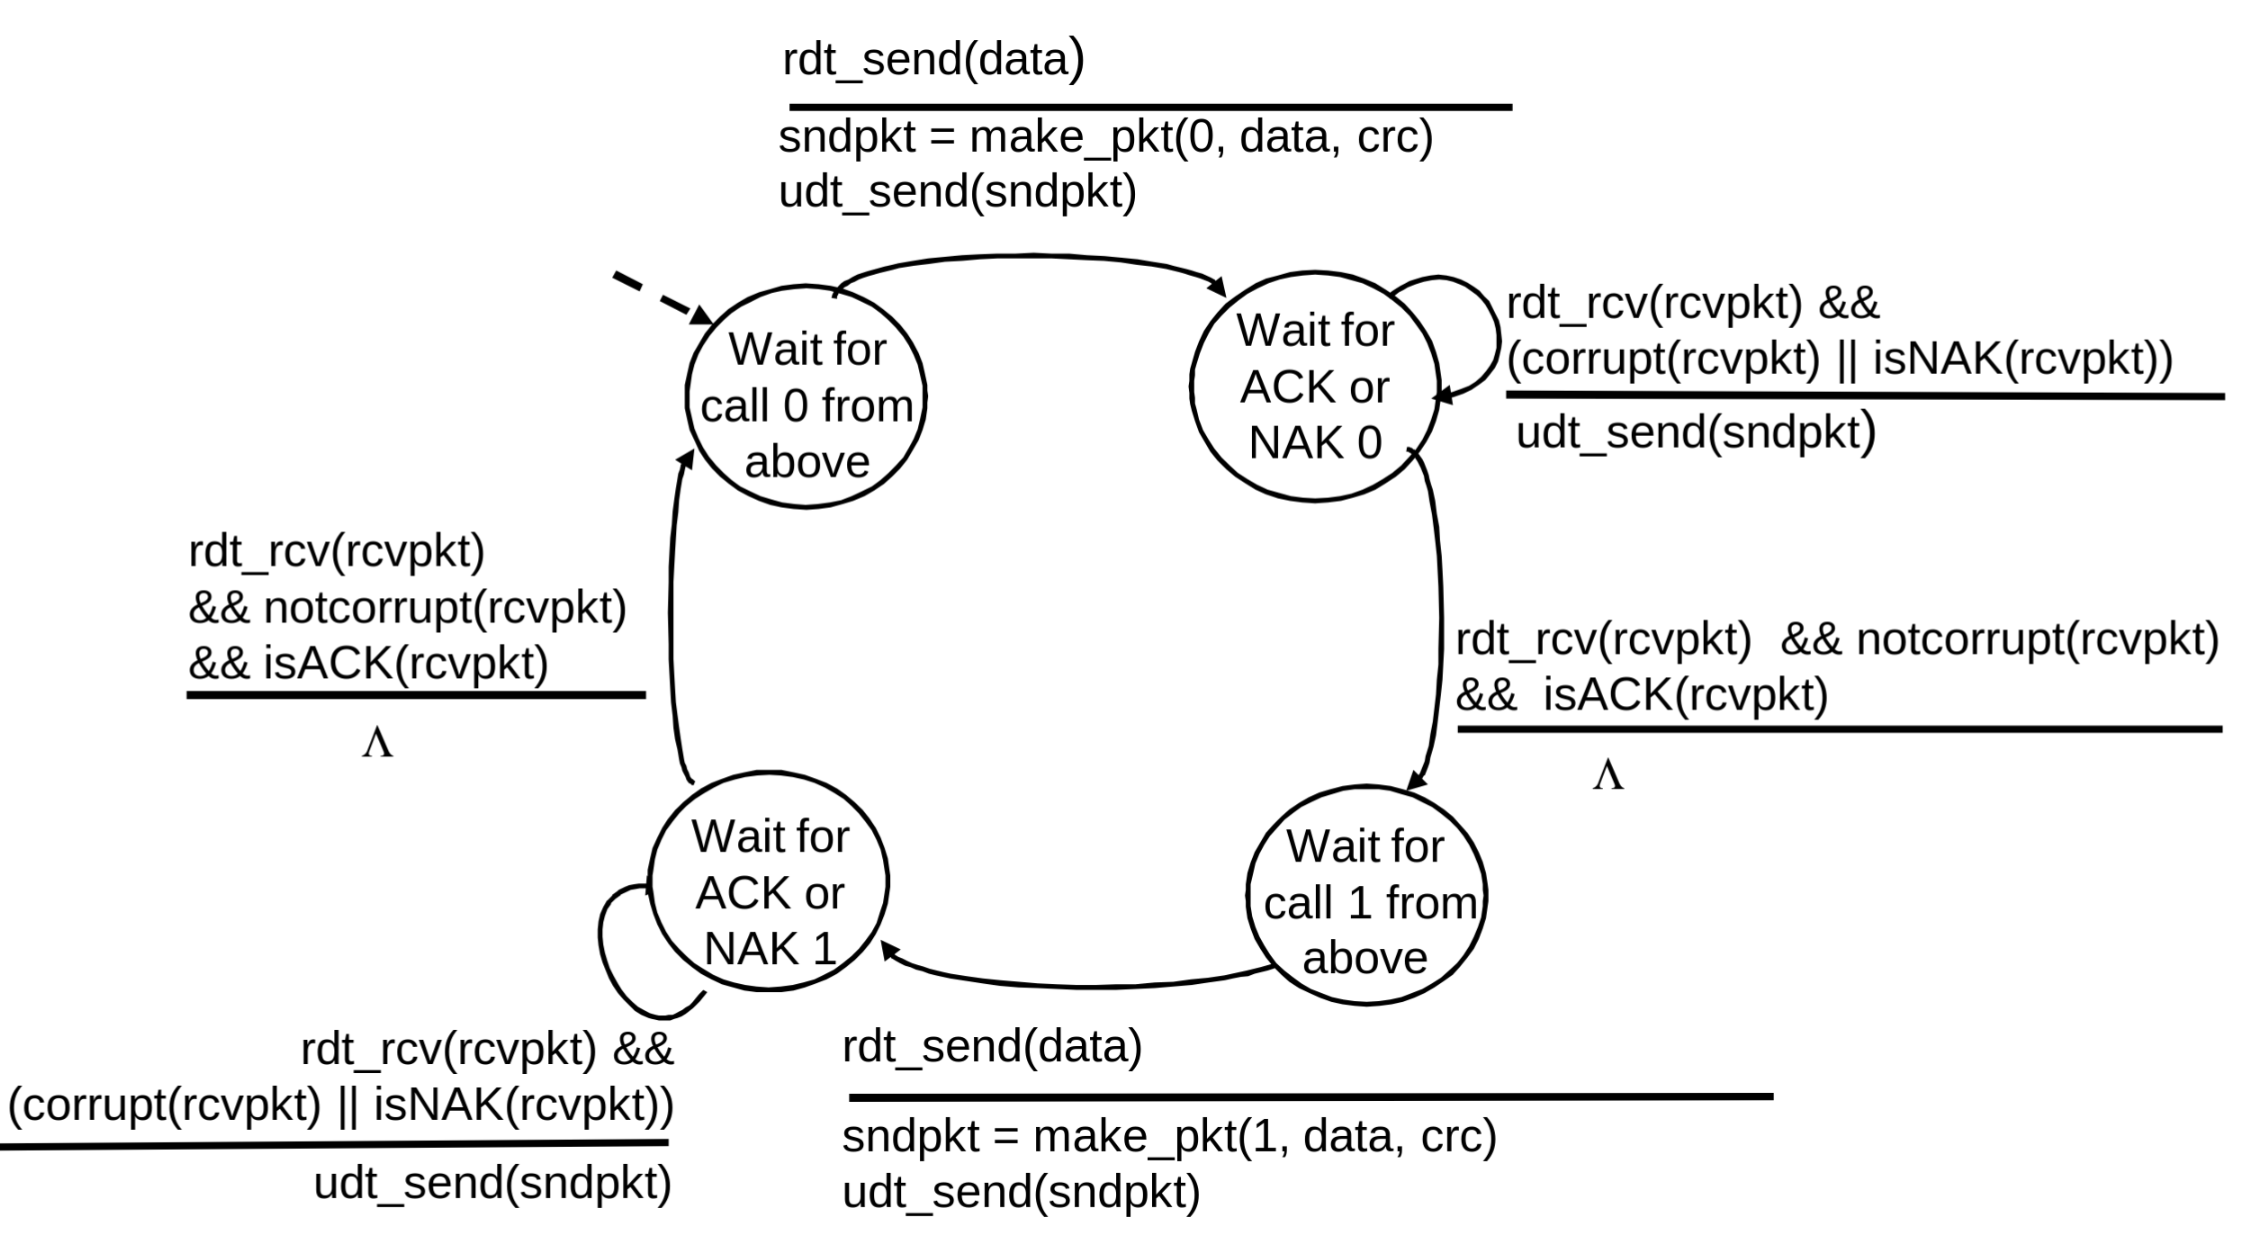
\includegraphics[scale=0.25]{../figures/rdt21fsm.png}
\end{center}

Quello che facciamo è:
\begin{itemize}
	\item Aspettare la chiamata dall'alto ed inviare il primo pacchetto (con numero di sequenza 0);
	\item Continuare ad inviare il pacchetto finche non si riceve un ACK non corrotto;
	\item Aspettare la chiamata dall'alto ed inviare il secondo pacchetto (con numero di sequenza 1);
	\item Di nuovo, continuare ad inviare il pacchetto finche non si riceve un ACK non corrotto.
\end{itemize}

Questo andamento si ripete in maniera ciclica.

\newpage

Il ricevitore potrà a questo punto eseguire il seguente automa:
\begin{center}
	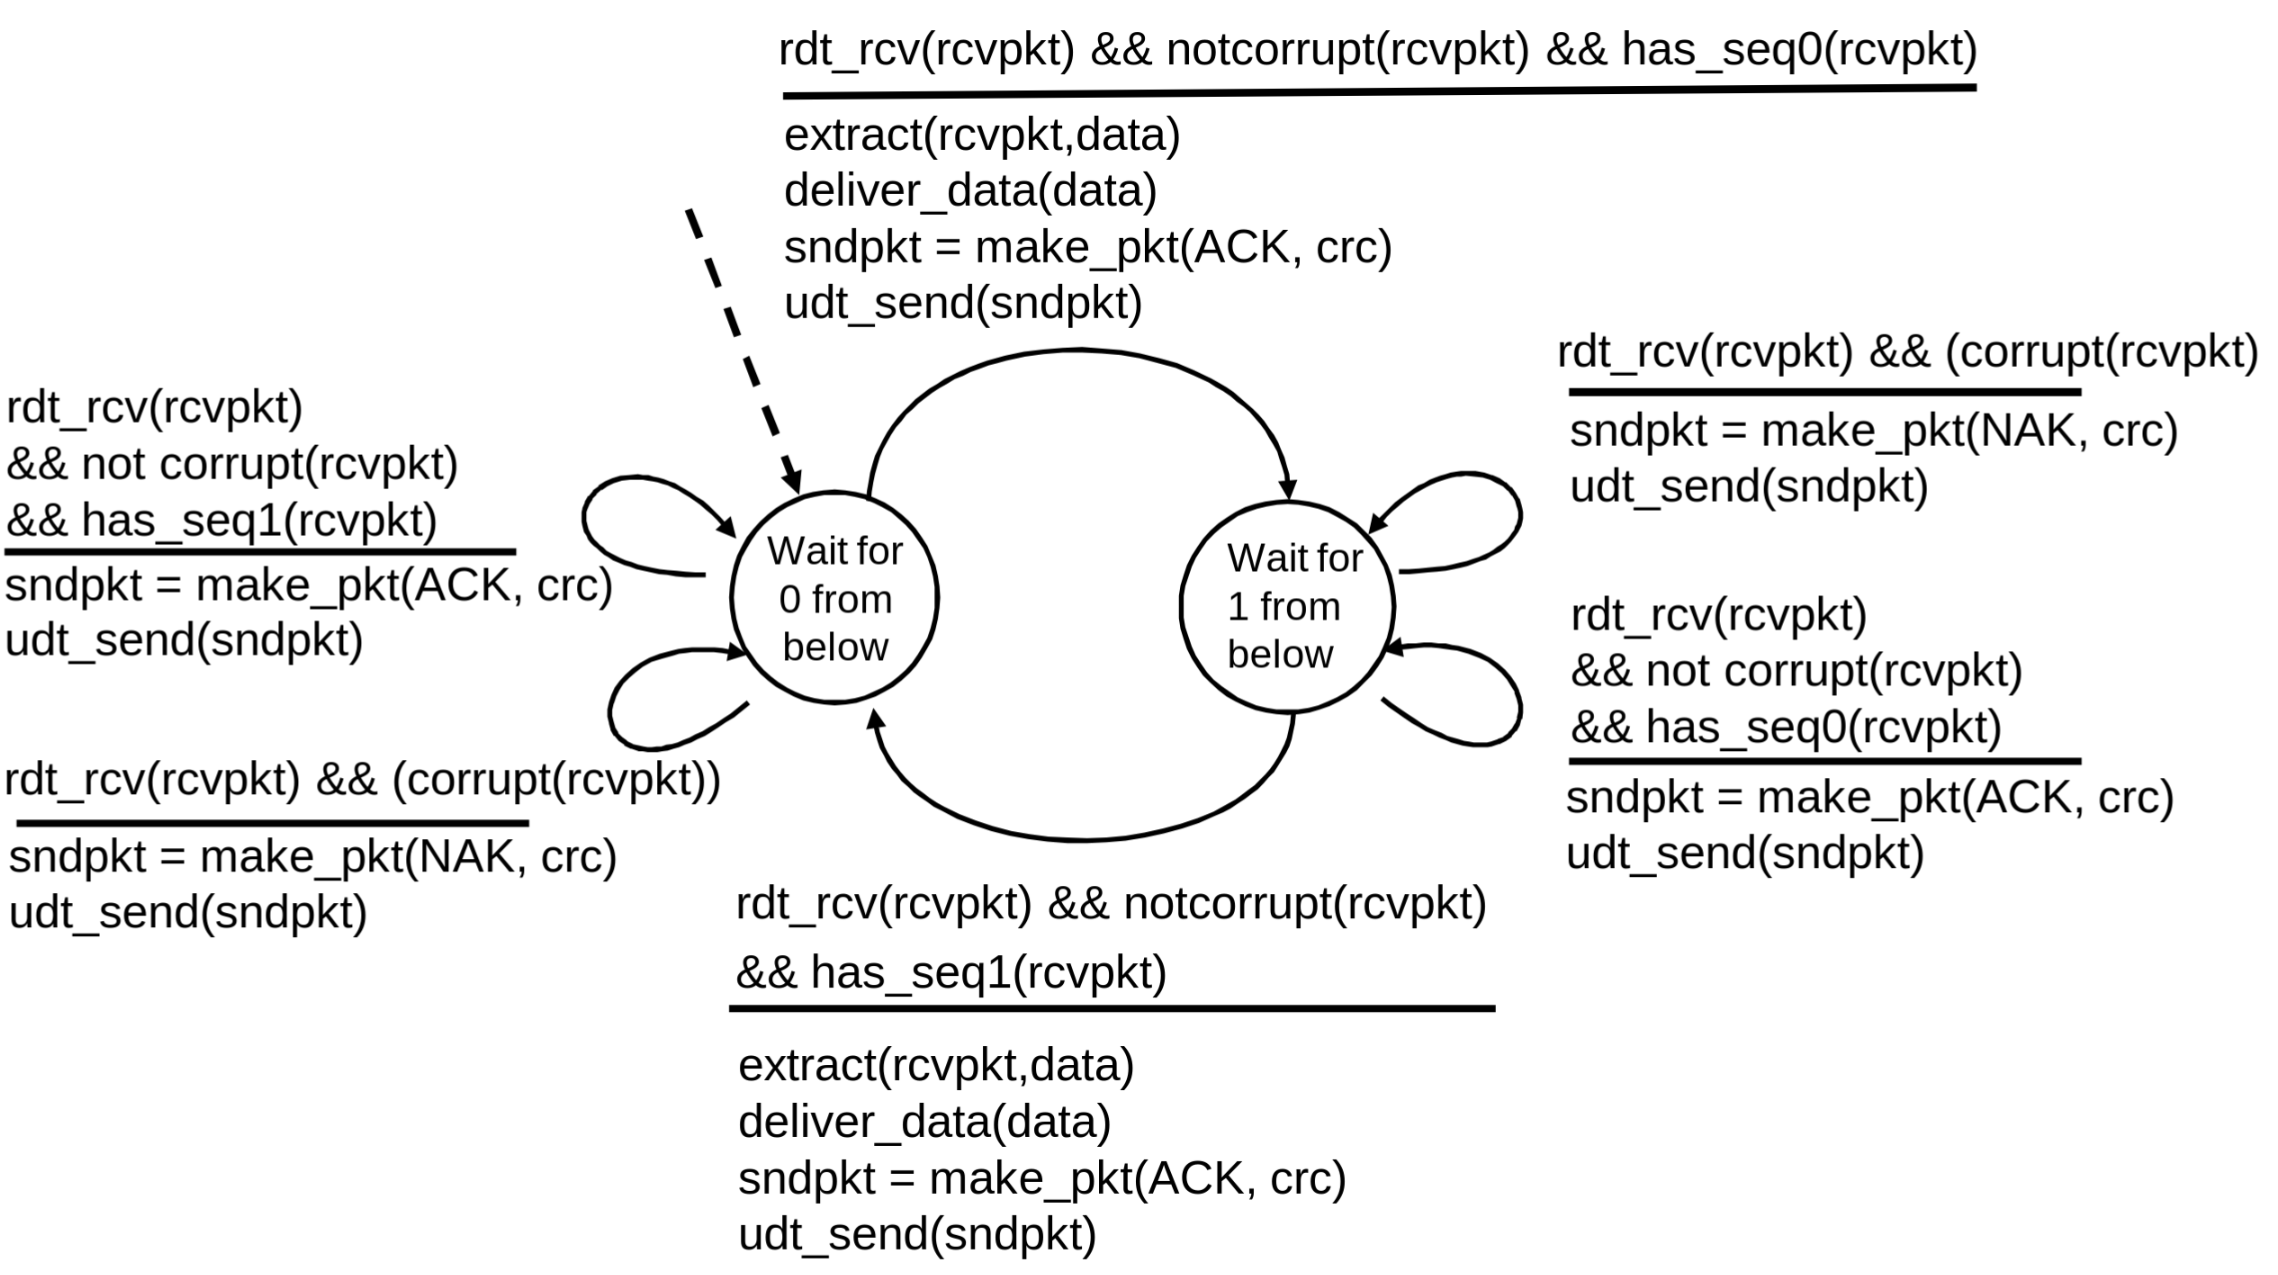
\includegraphics[scale=0.25]{../figures/rdt21fsm2.png}
\end{center}

In questo caso il flusso è:
\begin{itemize}
	\item Si aspetta per il primo pacchetto (dopo la chiamata dal basso), si invia un pacchetto ACK nel caso questo arrivi integro e con numero di sequenza 0, NAK altrimenti;
	\item Si aspetta il secondo pacchetto, comportandoci in maniera analoga, ma verificando che il numero di sequenza sia 1.
\end{itemize}

\subsubsection{RDT 2.2}
Si può semplificare l'approccio sopra riportato guardando semplicemente agli ACK e ai numeri di sequenza: in questo caso il ricevitore deve solo inviare ACK per gli ultimi pacchetti ottenuti integri.
ACK per pacchetti già trasmessi verrano interpretati dal trasmettitore come avevamo interpretato i NAK fino ad ora.

\newpage
In questo caso le macchine a stati si modificano come segue:
\begin{center}
	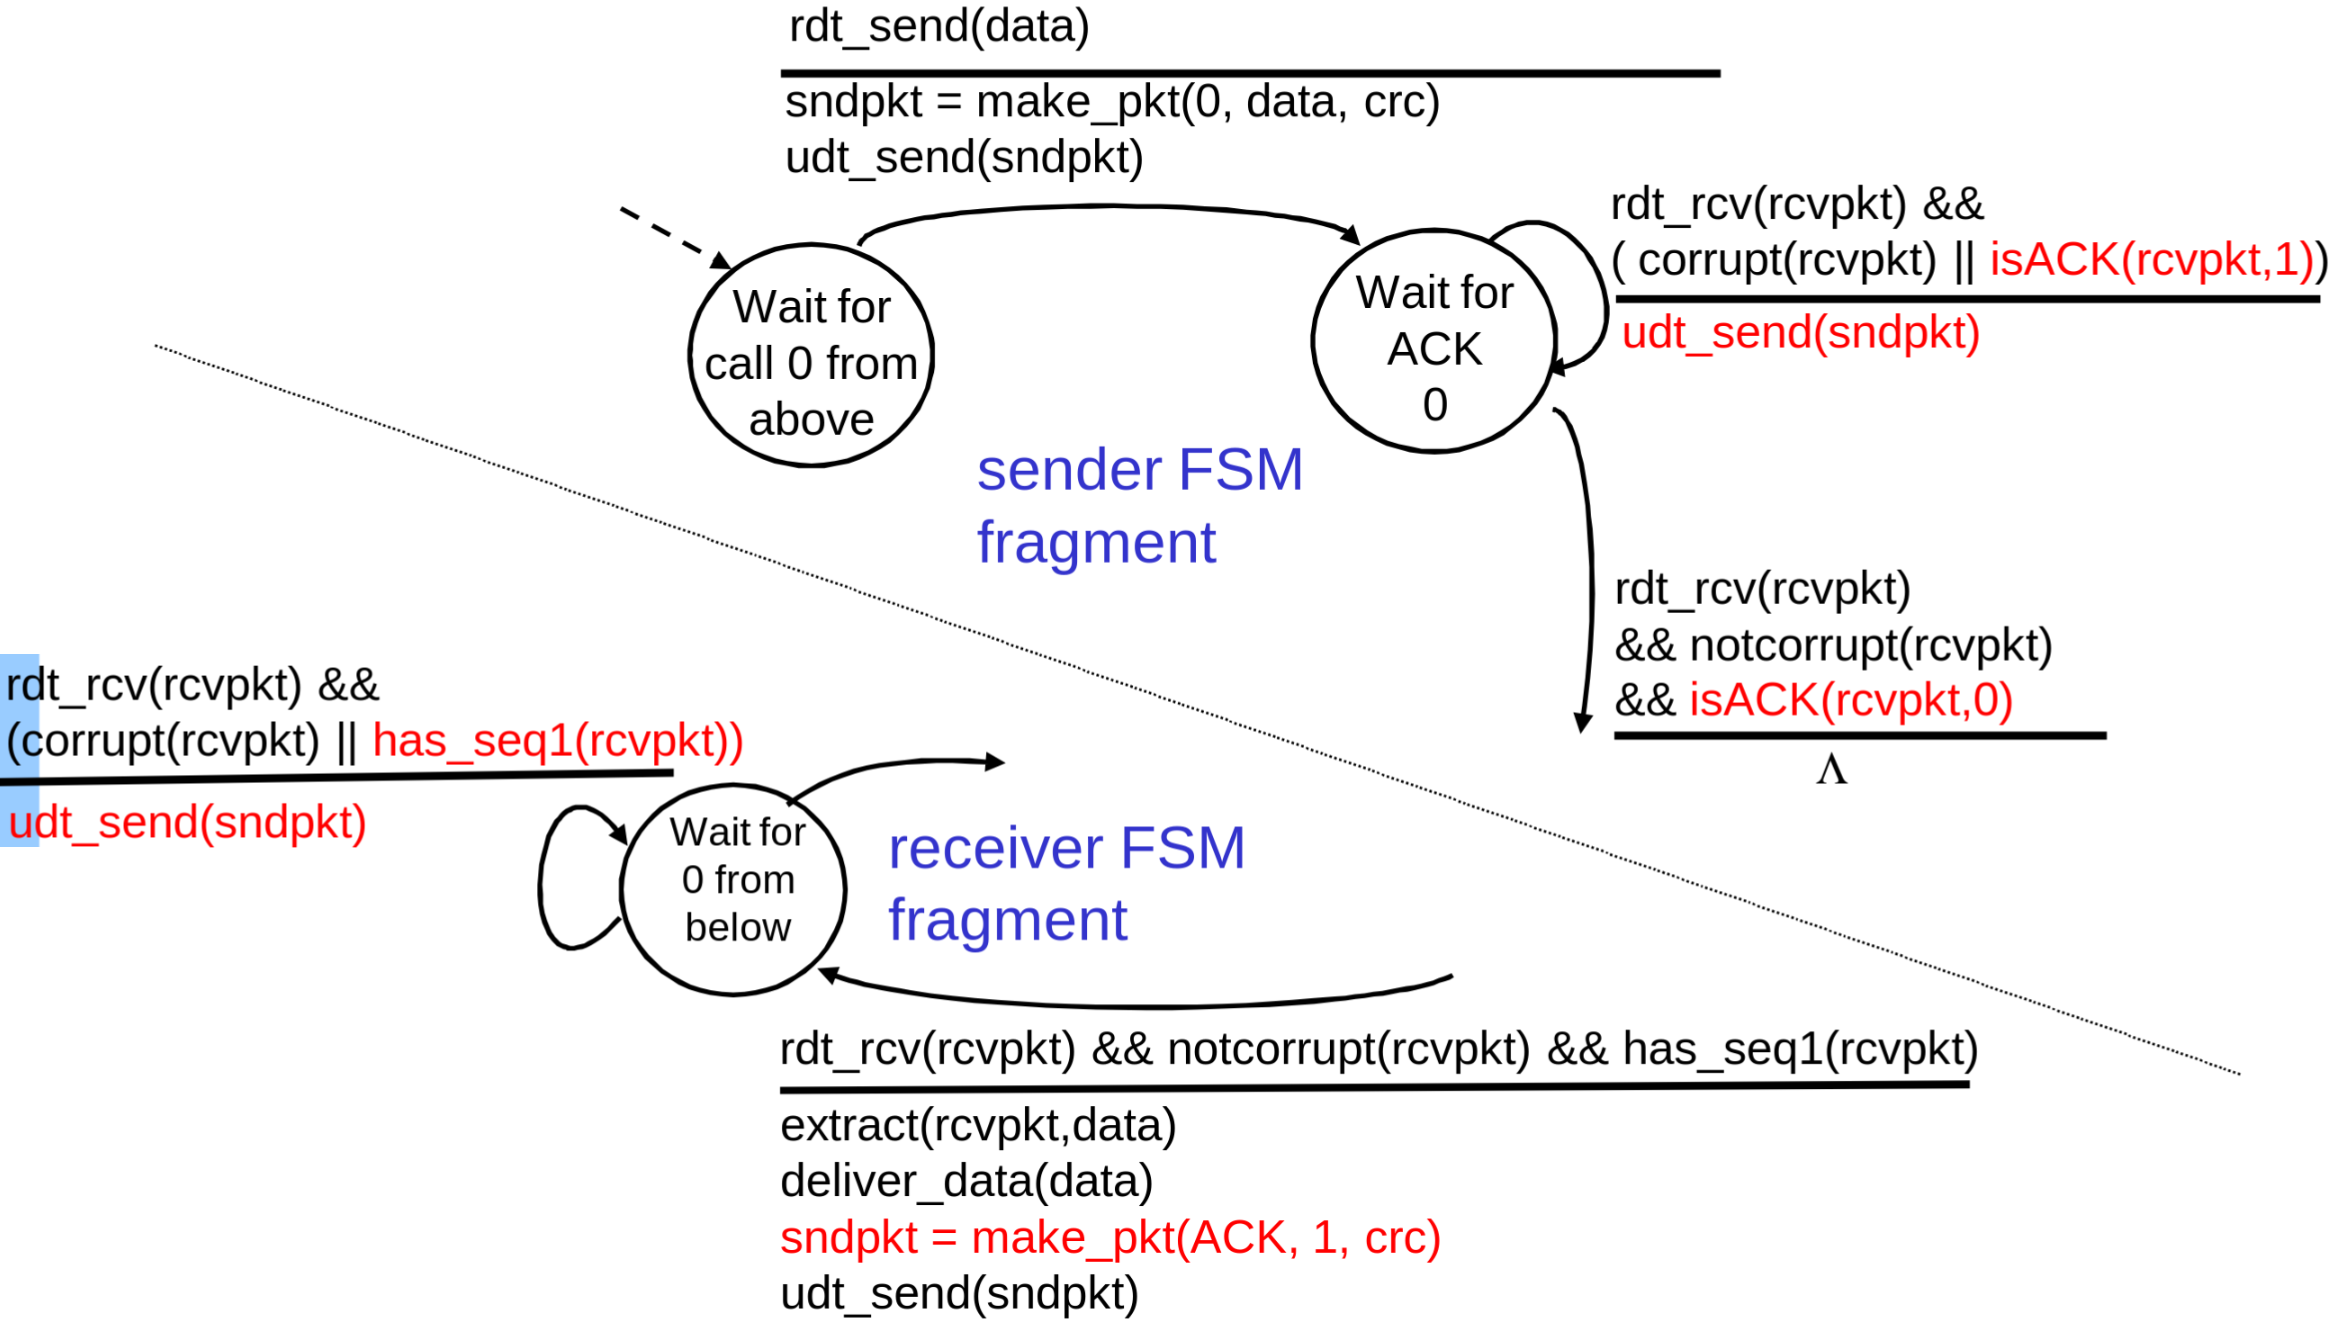
\includegraphics[scale=0.25]{../figures/rdt22fsm.png}
\end{center}

\subsection{RDT 3.0}
Facciamo una nuova assunzione sui canali: diciamo che il canale sottostante può anche \textit{perdere} (sia data che ACK), mentre prima poteva solo avere errori.

In questo caso potremo sfruttare checksum, numeri di sequenza, ACK e ritrasmissioni, ma non basterà completamente a risolvere il problema.

Un primo approccio potrebbe essere, lato tramsettitore, di aspettare un tempo ragionevole per l'arrivo dell'ACK da parte del ricevitore.
\textit{"Ragionevole"} può avere molti significati: assumiamo che il tempo sia tarato sul round-trip-time del link corrente.
Dopo che questo tempo passa, quindi, si procede col reinvio del pacchetto:
\begin{itemize}
	\item Se il pacchetto non era arrivato, il problema è risolto;
	\item Se il pacchetto era già arrivato e si era perso l'ACK, il ricevitore riceverà pacchetti duplicati: i numeri di sequenza risolvevano già questo prolema. Chiaramente, il ricevitore dovrà specificare il numero di sequenza del pacchetto per cui sta facendo ACK.
\end{itemize}

\newpage

La macchina a stati del trasmettitore con questo approccio è:
\begin{center}
	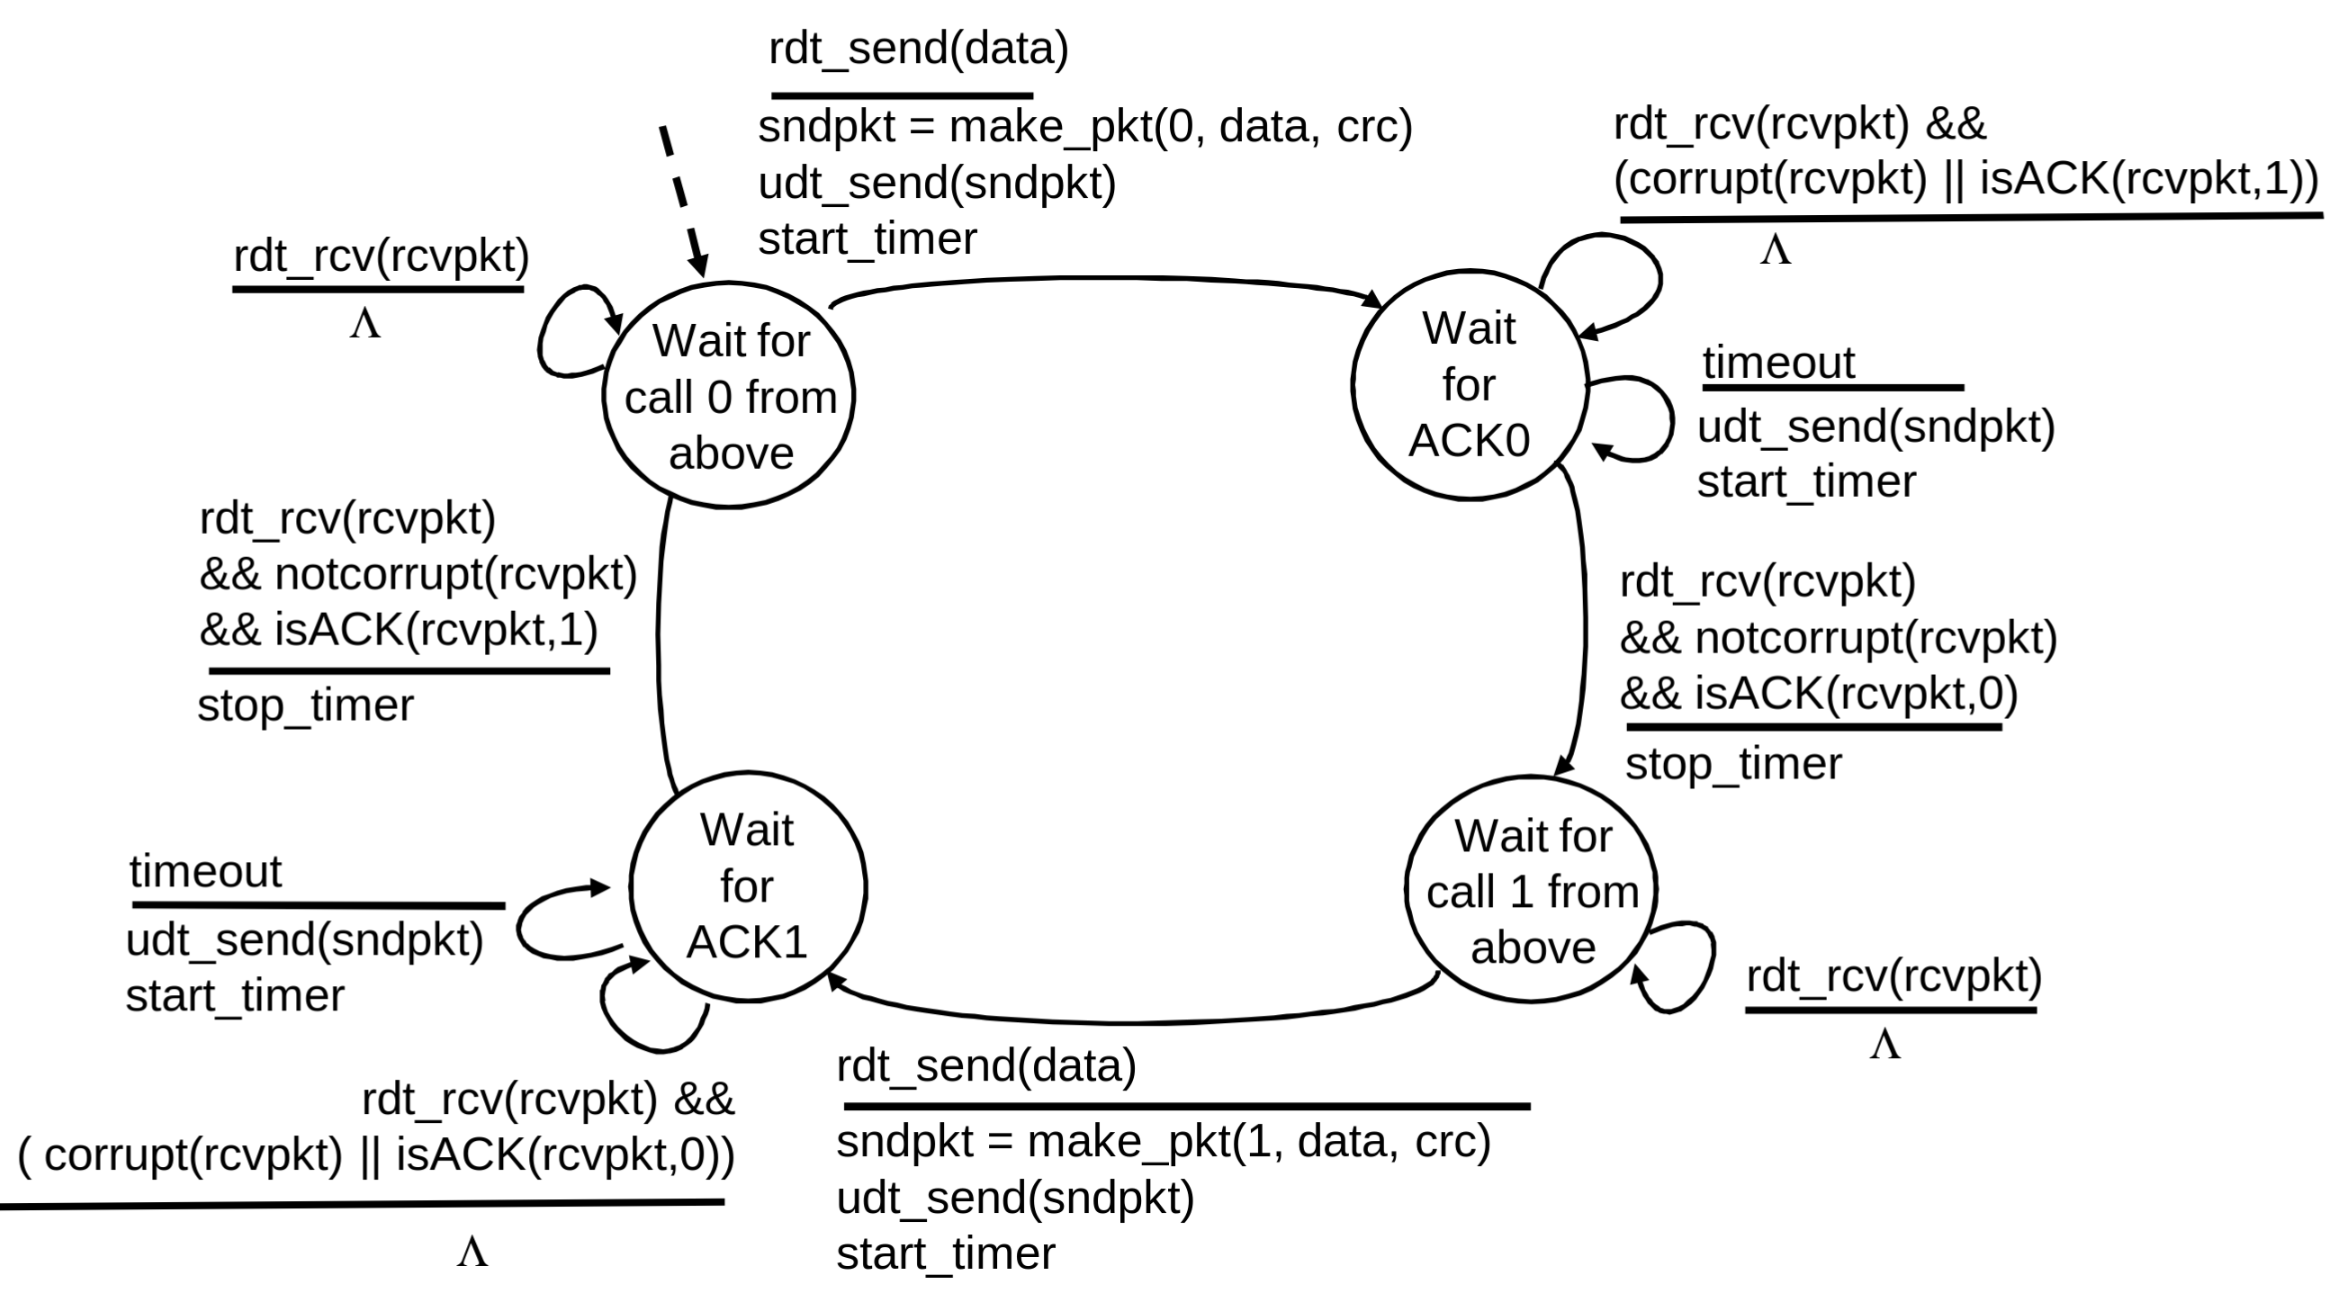
\includegraphics[scale=0.25]{../figures/rdt3fsm.png}
\end{center}

Ciò che facciamo è analogo a RDT 2.1, con la differenza che:
\begin{itemize}
	\item Quando inviamo il pacchetto, facciamo partire un timer;
	\item Se il timer fa timeout durante la fase di attesa per l'ACK, si reinvia il pacchetto al numero di sequenza corrente e si fa ripartire il timer.
\end{itemize}

Notiamo come si adotta un'approccio \textit{lazy} ai pacchetti ACK corrotti o per pacchetti con numero di sequenza sbagliato (quello che interpretavamo come NAK): in questo caso si ignorano e ci si affida al timeout (che prima o poi arriverà) per effettuare il reinvio.

Lato ricevitore, nulla cambia rispetto a RDT 2.2.

\subsubsection{Prestazioni di RDT 3.0}
Facciamo alcune note sulle \textbf{prestazioni} che riusciamo ad ottenere.

Sia $U_\text{sender}$ l'\textbf{utilizzazione tramsettitore}, cioè la frazione di tempo sul RTT usata dal trasmettitore in fase di invio effettivo del pacchetto.

Se assumiamo di avere un link da 1 Gbps, 15 ms di ritardo di propagazione e di dover trasmettere un pacchetto da 8000 bit.
Il tempo per trasmettere un pacchetto sul canale sarà allora circa:
$$
D_{\text{trans}} = \frac{L}{R} = \frac{8000}{1000} = 8 \, \text{ms}
$$

In condizioni ideali, quindi, avremo che dovremo inviare un pacchetto e aspettare un ACK (spedito in tempo trascurabile): questi sono due viaggi sul link (quindi un RTT dato dal due volte il ritardo di propagazione) e il tempo di trasmissione del pacchetto vero e proprio.
Si ha quindi:
$$
U_{\text{sender}} = \frac{ L/R }{ RTT + L/R } = \frac{0.0008}{30 + 0.0008} = 0.00027
$$

Cioè l'utilizzazione è terribile: del tempo che impieghiamo a trasmettere un pacchetto, meno dell'$0.001\%$ è effettivamente usato per trasmettere i dati che ci interessano!
Il problema è chiaramente che passiamo molto tempo ad \textit{aspettare}, quando potremmo avvantaggiarci con l'invio dei pacchetti successivi.

\subsection{Pipelining}
Il \textbf{pipelining} è un meccanismo attraverso il quale il trasmettitore può inviare più pacchetti in massa, senza aver ancora ricevuto l'ACK.
Lo poniamo come alternativa allo \textit{stop-and-wait} visto finora.

Riprendendo i conti della scorsa sezione, prendiamo ad esempio di inviare 3 pacchetti invece di 1 per ciclo di ACK. In questo caso si avrà:
$$
U_{\text{sender}} = \frac{ 3 L/R }{ RTT + L/R } = \frac{0.0024}{30 + 0.0008} = 0.00081
$$
che non è molto ma è già di più.

Chiaramente questo comporta delle complicazioni lato ricevitore: dovremmo prevedere la bufferizzazione dei pacchetti in entrata, e ingrandire il contatore del numero di sequenza (2 valori non basteranno più).

Trascurando quanto avviene lato ricevitore, una domanda interessante è \textit{quanti} pacchetti possiamo anticipare prima dell'ACK successivo: dovremmo riempire la finestra del $RTT$ con più tramissioni (ciascuna occupante tempo $\frac{L}{R}$), cioè inviare un numero di pacchetti al massimo pari a:
$$
N = \frac{RTT}{L / R}
$$

Approcci di questo tipo vengono detti a \textbf{sliding window} (\textit{"finestra scorrevole"}), in quanto prendono buffer scorrevoli sul blocco di pacchetti da inviare.

\subsubsection{Recupero errori in pipelining}
Abbiamo visto che, se vogliamo implementare un protocollo in pipelining, dobbiamo adoperare alcune soluzioni tecniche:
\begin{itemize}
	\item Buffering al trasmettitore dei pacchetti da inviare;
	\item Buffering al ricevitore dei pacchetti da ricevere, senza nessuna assicurazione che questi vengano ricevuti in ordine (serve il numero di sequenza);
	\item Un contatore per il numero di sequenza più grande al ricevitore.
\end{itemize}

Le specifiche di queste soluzioni vengono definite dal protocollo per il recupero dagli errori che adottiamo. 
Ne vederemo i 2 principali, che sono \textbf{go-back-N} e \textbf{selective-repeat}.

\subsubsection{Go-back-N}
In questo caso il trasmettitore mette fino a $N$ pacchetti senza ACK in pipeline.
Al ricevitore viene permesso solo di inviare ACK cumulativi: non effettua ACK se perde uno degli $N$ pacchetti.
Il trasmettitore mantiene quindi un timeout per gli ultimi $N$ pacchetti inviati: se il timer scade reinvia tutti gli $N$ pacchetti.

\par\smallskip

Lato implementativo si ha quindi che il trasmettitore spedisce fino a $N$ pacchetti consecutivi sulla pipeline.
Il ricevitore invia da parte sua ACK consecutivi al pacchetto con numero di sequenza più alto ricevuto fino a quel momento (se bufferizzare o meno i pacchetti che non combaciano col numero di sequenza aspettato è una scelta implementativa).

Quando il primo pacchetto della sequenza spedita viene ricevuto, il trasmettitore sposta in avanti la sua finestra e spedisce il successivo, spostandosi così lungo il blocco di pacchetti.

Se un pacchetto viene perso, il trasmettitore aspetta senza spostare la finestra: prima o poi scatterà il timeout del pacchetto perso e verrà reinviato.
Lato ricevitore, possiamo aspettarci che questo passerà lo stesso intervallo temporale a inviare ACK sempre sull'ultimo pacchetto valido (con numero di sequenza consecutivo) ricevuto, e che il trasmettitore abbia ignorato tale ACK in quanto ascolta solo l'ACK più grande ricevuto.

\subsubsection{Selective repeat}
In questo caso il trasmettitore invia $N$ pacchetti senza ACK in pipeline (come sopra).
La differenza è che il ricevitore invia ACK per ogni pacchetto: il trasmettitore deve quindi mantenere un timer per ogni pacchetto inviato, e nel caso questo timer faccia timeout inviare solo il pacchetto corrispondente.

Questo approccio è chiaramente più efficiente: si ritrasmettono solo i pacchetti persi, a costo di un'implementazione più costosa sia lato trasmettitore (dobbiamo mantenere più timer) che ricevitore (dobbiamo inviare ACK separati per ogni pacchetto).

Il caso in cui approcci come il go-back-N vengono comunque usati è quello di dispositivi \textit{constraining} (come quelli che si usano nell'IoT): questi hanno prestazioni meno soddisfacenti e quindi impongono di usare protocolli meno efficienti.

\end{document}
